\section{Extension to multiple data sources}\label{sec_same}

%We begin by considering the case where all tasks have the same sample size and feature covariates, that is, $n_i = n$ and $X^{(i)} = X\in\real^{n\times p}$ for all $i = 1, \dots, t$.
%We provide a sharp generalization error bound of hard parameter sharing estimators.

%Hard parameter sharing is a commonly used architecture in multi-task learning. However, there have been few theoretical results on the performance of the HPS estimators in high-dimensional multi-task learning. In this section, we extend our results on the predication loss of the HPS estimator to a multi-task linear regression, where all tasks have the same covariates. We make this extension for the following reasons. First, its restriction to the two-task case provides a rare example where the output layers $A_1$ and $A_2$ can be characterized exactly. Second, the proof of the multi-task case is no harder than the two-task case, but it can provide much clearer geometric intuition  as we will discuss below. Third, the corresponding multi-task setting is prevalent in applications of multi-task learning to image classification, where there are multiple prediction labels/tasks for every image \cite{chexnet17,EA20}. Finally, it provides useful insights into a more general theory of multi-task learning, which we will explore in greater details in future works.
%It is not hard to extend the above result to the cases with more than two tasks. {\cor For the general case, we study them in a future work.}

%Suppose we have $t$ datasets.
%For each dataset $i$ from $1$ to $t$, let $n_i$ denote its sample size.
%Let $X^{(i)} \in \real^{n_i \times p}$ denote dataset $i$'s feature covariates.
%We assume that the label vector $Y^{(i)} \in \real^{n_i}$ for $X^{(i)}$ follows a linear model plus random noise.
%We study the standard hard parameter sharing architecture:
%a shared feature representation layer $B\in\real^{p\times r}$ for all datasets and a separate output layer $A_i \in \real^r$ for every dataset $i$.
%See Figure \ref{fig_intro_arch} for an illustration.
%The width of $B$, denoted by $r$, plays an important role in regularization.
%As observed in Proposition 1 of \cite{WZR20}, if $r \ge t$, there is no regularization effect.
%Hence, we assume that $r < t$ in our study.
%For example, when there are only two tasks, $r = 1$ and $B$ reduces to a vector whereas $W_1, W_2$ become scalars.
%We study the following minimization problem:
%	\item Separate each dataset $(X_i, Y_i)$ randomly into a training set $(X_i^{tr}, Y_i^{tr})$ and a validation set $(X_i^{val}, Y_i^{val})$.
%	The size of each set is described below.
%	\item Learn the shared layer $B$: minimize the training loss over $B$ and $W_1, \dots, W_t$, leading to a local minimum of $B$ that depends on $W_1, \dots, W_t$, denoted by $\hat{B} = \hat{B}(W_1, \dots, W_t)$.
%\vspace{-0.1in}
%\begin{align}\label{eq_mtl}
%			f(A, B) = \sum_{i=1}^t \norm{X^{(i)} B A_i - Y^{(i)}}^2,
%\end{align}
%\vspace{-0.05in}
%where $A = [A_1, A_2, \dots, A_t] \in \real^{r \times t}$.

Our setup and the results in Section \ref{sec_main} are both for transferring from one data source.
This section extends our setup to transfer learning from multiple data sources.
We focus on a natural setting where all the tasks have the same covariates but different labels.

\paragraph{Data model.} Suppose we have $t$ datasets whose sample sizes are all equal to $n$ and whose feature covariates are all equal to $X \in \real^{n \times p}$. The label vector of the $i$-th task follows a linear model
\begin{align}
    Y^{(i)} = X \beta^{(i)} + \varepsilon^{(i)}, \text{ for } i=1, 2,\cdots, t.
\end{align}
We assume several standard conditions on $X$ and each of $\varepsilon^{(i)}$.
First, $X = Z\Sigma^{1/2}$ is a random matrix satisfying the same assumption as $X^{(2)}$ in Assumption \ref{assm_big1}.
%that is, $Z$ is an $n\times p$ random matrix with i.i.d. entries satisfying (\ref{assm1}) and \eqref{conditionA2}, $\Sig$ is a deterministic positive definite symmetric matrix satisfying \eqref{eigen} and \eqref{assm3}, and $\rho:=n/p$ satisfies \eqref{assm2}.
Second, every $\varepsilon^{(i)} \in \real^{n}$ is a random vector with i.i.d entries of mean zero, variance $\sigma^2$, and bounded moments as in equation \eqref{eq_highmoments}.
Finally, $\beta^{(i)} \in \real^{p}$ is a fixed vector independent from the other linear models, the feature covariates, and all noise vectors.

%\begin{figure*}[!t]
%	\centering
%	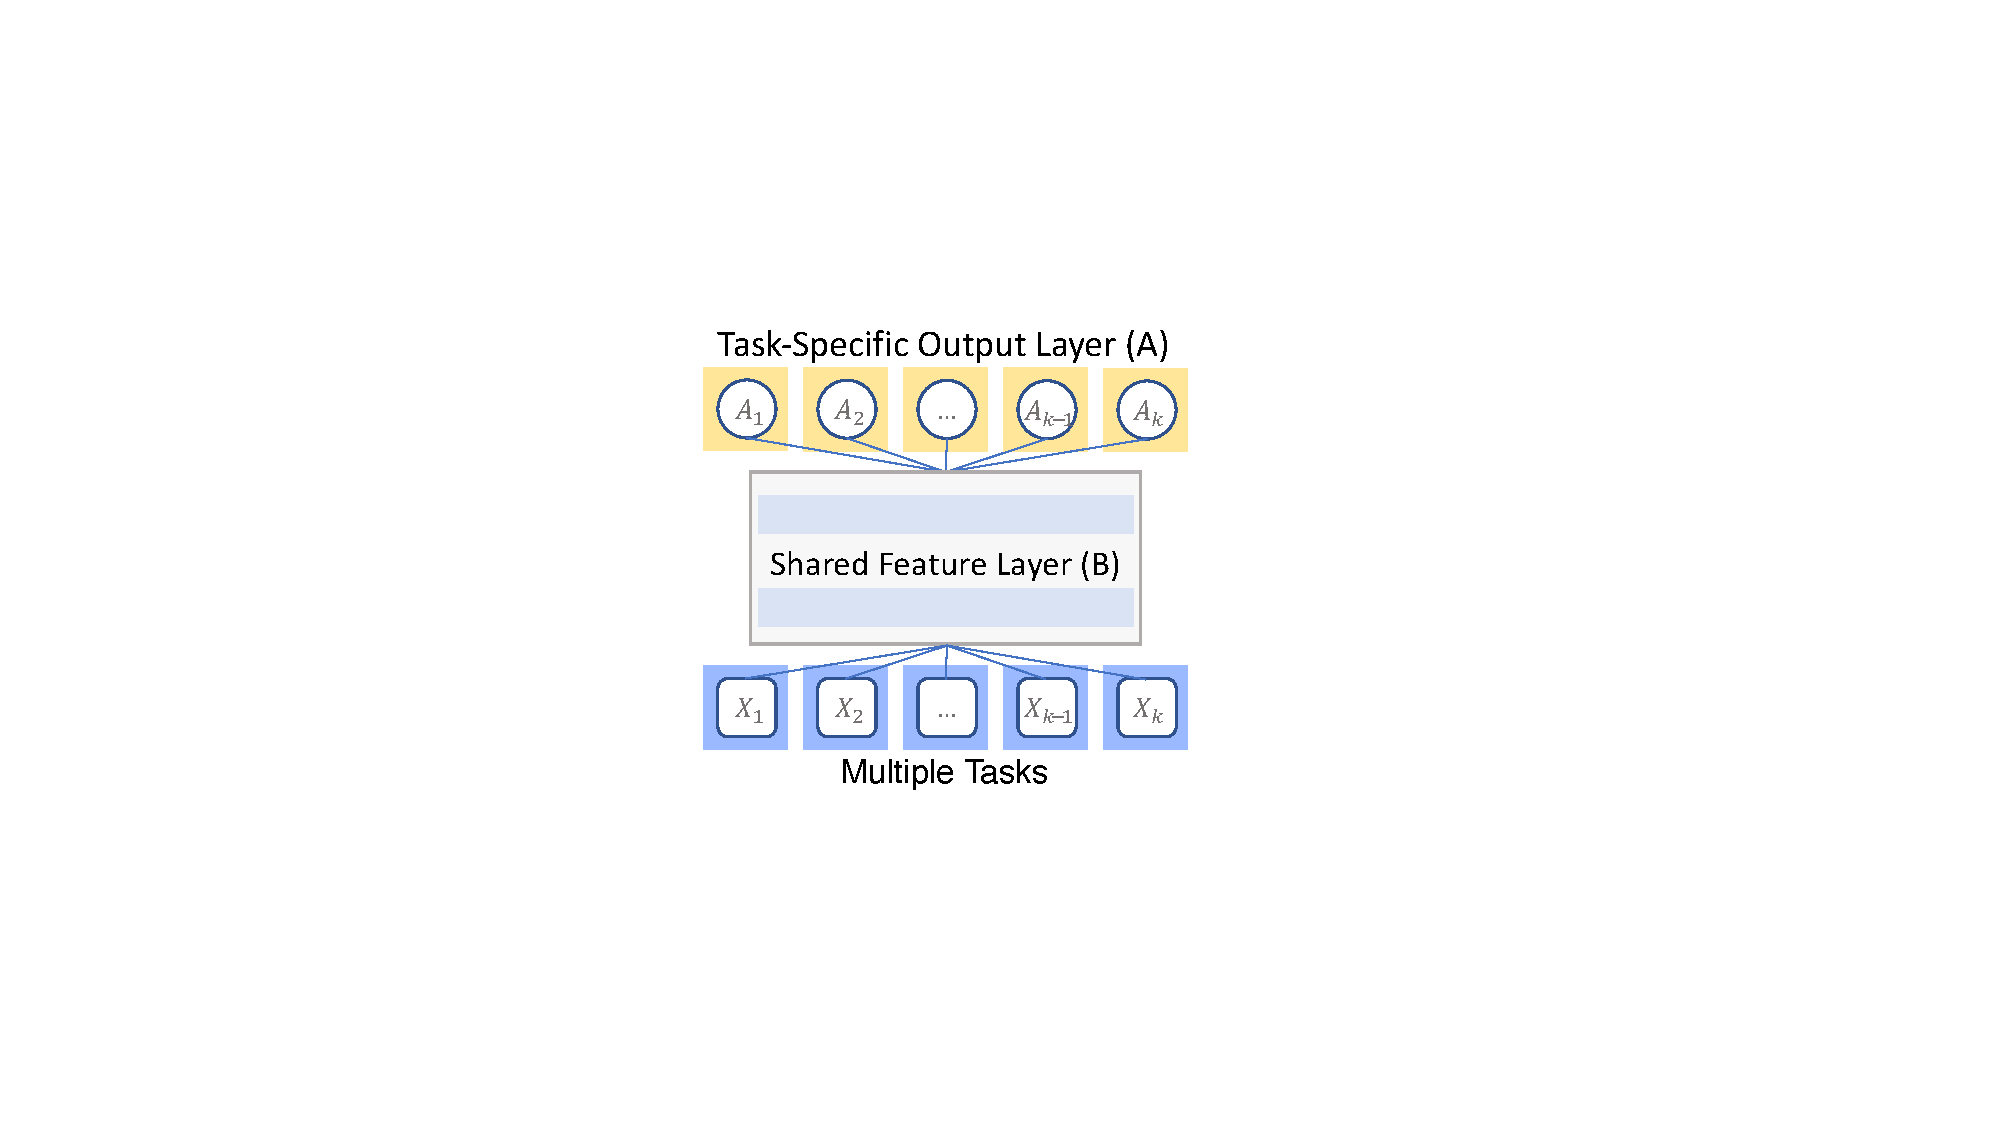
\includegraphics[width=0.3\textwidth,valign=t]{figures/mtl_model_arch.pdf}
%	\caption{A hard parameter sharing architecture}
%	\label{fig_intro_arch}
%\end{figure*}
%\begin{enumerate}
%	\item $X = Z \Sigma^{1/2} \in \real^{n\times p}$ for a positive semidefinite matrix $\Sigma\in \R^{p\times p}$, and every entry of $Z \in \real^{n \times p}$ is drawn independently from a one dimensional distribution with zero mean, unit variance, and constant $\varphi$-th moment for a fixed $\varphi > 4$.
%	\item every entry of $\varepsilon^{(i)} \in \real^{n \times t}$ is drawn indepdently from a one dimensional distribution with zero mean, variance $\sigma^2$, and bounded moment up to any order.\footnote{There exists a fixed function $C: \mathbb{N} \rightarrow \real^+$ such that for any $k \in \N$, the $k$-th moment is bounded by $C(k)$.}
%\end{enumerate}

\paragraph{Estimator.} We extend the two-layer linear neural network from equation \eqref{eq_hps} to combine multiple data sources as follows:
\begin{align}
	f(A, B) = \sum_{j=1}^t \bignorm{X B A_j - Y^{(j)}}^2, \label{eq_mtl_same_cov}
\end{align}
where $B \in \real^{p \times r}$ is a rank-$r$ shared feature representation layer, and $A := [A_1, A_2, \dots, A_t] \in \real^{r \times t}$ with $A_i \in \R^r$ being a separate output layer for task $i$. %Recall that $r$ is the width of $B$.
We will focus on cases with $r < t$.
Otherwise, the global minimum of $f(A, B)$ reduces to single-task learning, similar to Proposition \ref{prop_large_r} (details omitted).

Let $\hat A$ be the global minimizer of $g(A)$. Then $(\hat A,\hat B(\hat A))$ is the global minimizer of $f(A,B)$. We define the HPS estimator for task $i$ as $\hat \beta_i^{\MTL} := \hat B(\hat A) \hat A_i,$
%For an estimator $\hat{\beta}_i$ of task $i$, we are interested in
and its (out-of-sample) prediction loss as
\be\label{ith_loss} L_i(\hat{\beta}_i^{\MTL}) = \bignorm{\Sigma^{1/2} \left(\hat{\beta_i}^{\MTL} - \beta^{(i)}\right)}^2. \ee

	For the optimization objective  in \eqref{eq_mtl_same_cov}, using the local optimality condition over $B$, that is, $\frac{\partial f}{\partial B} = 0$, we obtain $\hat{B}$ as a function of $A$:
	\begin{align}
		\hat{B}(A) %&\define (X^{\top}X)^{-1} X^{\top} \bigbrace{\sum_{j=1}^t Y^{(j)} A_j^{\top}} (A  A^{\top})^{+} \nonumber \\
		&= (X^{\top} X)^{-1} X^{\top} Y A^{\top} (AA^{\top})^{+}, \label{eq_Bhat}
	\end{align}
	where $Y := [Y^{(1)}, Y^{(2)}, \dots, Y^{(t)}]$ and $(AA^{\top})^{+}$ denotes the pseudoinverse of $AA^{\top}$.
	%Here we have used that $X^{\top}X$ is invertible since $n > \rho \cdot p$ and $\rho > 1$ (cf. Fact \ref{fact_minv}).
	%\FY{Is $\dag$ a standard notation? It is a bad notation at least for me because $\dag$ is more often used as Hermitian conjugate. Wiki page uses $(AA^{\top})^{+}$ for pseudo-inverse.}
	Plugging $\hat{B}(A)$ into equation \eqref{eq_mtl_same_cov}, we obtain the following objective that only depends on $A$ (in matrix notation):
	\begin{align}\label{eq_mtl_output_layer}
		g(A) = \bignormFro{X (X^{\top}X)^{-1}X^{\top} Y A^{\top} (AA^{\top})^{+} A - Y}^2.
	\end{align}
%	Note that $A^{\top} (AA^{\top})^{+} A$ is a projection onto the subspace spanned by the rows of $A$. For simplicity, we write it into the form
%	$$A^{\top} (AA^{\top})^{+} A= U_A U_A^\top,$$
%	where $U_A \in \R^{t\times r}$ is a $t\times r$ partial orthonormal matrix (i.e. $U_A^\top U_A=\id_{r\times r}$). Hence we also denote the function $g(A)$ by $g(U_A)$.


\paragraph{Result.} Theorem \ref{thm_many_tasks}, shows that hard parameter sharing essentially approximates all tasks through a rank-$r$ subspace. To formalize this geometric intuition, as in the two-task case, we introduce the matrix $B^\star \define [{\beta}^{(1)},{\beta}^{(2)},\dots,{\beta}^{(t)}] \in \real^{p\times t}$ formed by the linear model parameters of all the $t$ tasks.
Let $A^{\star} {A^{\star}}^{\top}$ denote the best rank-$r$ subspace approximation of ${B^{\star}}^\top\Sigma B^{\star}$ (which can be regarded as the covariance of the task labels):
\begin{align}\label{eq_A_star}
	A^{\star} \define \argmin_{U\in\real^{t\times r} : U^{\top} U = \id_{r\times r}} \inner{U U^{\top}} {{B^{\star}}^{\top} \Sigma B^{\star}},
\end{align}
where $\langle \cdot ,\cdot \rangle $ denotes the Frobenius inner product between two matrices.
 To ensure that $A^{\star}$ is unique, we assume that the $r$-th largest eigenvalue of ${B^\star}^\top \Sigma B^\star$ is strictly larger than the $(r+1)$-th largest eigenvalue. Otherwise, $A^{\star}$ is not well-defined and Theorem \ref{thm_many_tasks} will give a null result.
 %$\lambda_{r+1}({B^\star}^\top \Sigma B^\star)$ is strictly smaller than $\lambda_{r}({B^\star}^\top \Sigma B^\star)$.
Let $a_i^{\star}:= A^{\star}{A^{\star}}^{\top} e_i \in\real^r$ denote the $i$-th column of $A^{\star}{A^{\star}}^{\top}$, where $e_i$ is the standard basis unit vector along $i$-th direction. Then we have the following result.


% $B^{\star} A^{\star} {A^{\star}}^{\top}$.
%Let $(\hat{A}, \hat{B})$ be the global minimizer of $f(A, B)$.
%Recall that the HPS estimator is defined as $\hat{\beta}_i^{\MTL} = \hat{B} \hat{A}_i$.
%Our result is stated as follows.

\begin{theorem}\label{thm_many_tasks}
%Suppose $X=Z\Sigma^{1/2}\in \R^{n\times p}$ satisfy Assumption \ref{assm_secA1} with $\rho:=n/p>1$ being some fixed constant. Consider data models  $Y_i = X\beta_i + \varepsilon_i$, $i=1,2,\cdots, t$, where $\e_i\in \R^{n}$ are random vectors with i.i.d. entries with mean zero, variance $\sigma^2$ and all moments as in \eqref{assmAhigh}. Moreover, assume that $X$, $\beta_i$ and $\e_i$ are all independent of each other.
	%Let $n = c \cdot p$.
	%Let $X\in\real^{n\times p}$ and $Y_i = X\beta_i + \varepsilon_i$, for $i = 1,\dots,k$.
%	Consider $t$ data models $Y_i = X\beta_i + \varepsilon_i$, $i=1,2,\cdots, t$, where $X$ has covariance matrix $\Sigma$, and the entries of $\e_i$ are i.i.d. with mean zero and variance $\sigma^2$.gT
	%that satisfy Assumption \ref{assm_secA2} in the appendix.
	%Assume that $n > \rho \cdot p$ for a fixed constant $\rho > 1$.
	%Let $c_{\varphi}$ be any fixed value within $(0, \frac{\varphi-4}{2\varphi})$.
%	Let $L(B^{\star}a_i^{\star}): = \norm{\Sigma^{1/2} (B^{\star} a_i^{\star}- \beta^{(i)})}^2$.
%Suppose $X\in \R^{n\times p}$ is an $n\times p$ random matrix satisfying the same assumptions as $X^{(1)}$ and $X^{(2)}$ in Assumption \ref{assm_big1}, and $\rho:=n/p$ satisfies \eqref{assm2}.
Suppose the above multi-task setting holds. Let $c>0$ be an arbitrary (small) constant. Then for any task $i = 1,  \cdots, t$, we have that with high probability,
\be\label{minimizer_beta}
\left\|  \hat A^{\top} (\hat A\hat A^{\top})^{+} \hat A - A^\star {A^\star}^\top\right\|_F  \le \left[ \frac{ n^{-1/2+2/\varphi+c}  \|{B^{\star}}^{\top}\Sigma B^{\star}\|  + n^{-1/2+c} \sigma^2 }{\lambda_r - \lambda_{r+1} }\right]^{1/2} ,
\ee
where $\lambda_r $ and $\lambda_{r+1}$ are respectively the $r$-th and $(r+1)$-th largest eigenvalues of ${B^\star}^\top\Sigma B^\star$. Moreover, the prediction loss of the HPS estimator $\hat{\beta}_i^{\MTL}$ satisfies that  with high probability,
	\begin{align}
		& \bigabs{L_i(\hat{\beta}_i^{\MTL}) - L_i(B^{\star}a_i^{\star}) -\frac{p\sigma^2}{n-p}  \norm{a_i^{\star}}^2  } \nonumber\\
		& \le  \left[ \frac{  n^{-1/2+ 2/\varphi +c}   \norm{{B^\star}^\top\Sigma B^\star} +n^{-1/2+c}  \sigma^2} {\lambda_r  - \lambda_{r+1} }\right]^{1/2}  \left(\norm{{B^\star}^\top\Sigma B^\star}+  \sigma^2\right). \label{Li_multi1}
		%\le n^{-\frac{c_{\varphi}}2} \cdot \frac{\bigbrace{ \norm{\Sigma^{1/2} B^{\star}}^2+  \sigma^2} \cdot (\bignormFro{\Sigma^{1/2} B^{\star}}^2 + \sigma^2 t)} {\lambda_r ({B^\star}^\top \Sigma B^\star)- \lambda_{r+1}({B^\star}^\top \Sigma B^\star)},
	\end{align}
	%where $\lambda_r({B^\star}^\top\Sigma B^\star)$ and $\lambda_{r+1}({B^\star}^\top\Sigma B^\star)$ are respectively be the $r$-th and $(r+1)$-th largest eigenvalue of ${B^\star}^\top\Sigma B^\star$.
%	where $C_1: = \frac{\bignormFro{\Sigma^{1/2} B^{\star}}^2 + \sigma^2 t}{\lambda_r ({B^\star}^\top \Sigma B^\star)- \lambda_{r+1}({B^\star}^\top \Sigma B^\star)}$. %and $C_2 :=  C_1\cdot \norm{\Sigma^{1/2} B^{\star}}$.
Finally, we have a better bound for the averaged prediction loss:  with high probability,
\begin{align}
&\left|\frac{1}{t}\sum_{i=1}^t L_i(\hat{\beta}_i^{\MTL}) - \frac1t\bignorm{\Sigma^{1/2} B^{\star} (A^\star {A^\star}^{\top} - \id_{t\times t})}_F^2 - \frac{p \sigma^2}{n-p}\cdot \frac{r}{t}  \right| \nonumber \\
 &\le n^{-1/2+2/\varphi+c}  \norm{{B^\star}^\top\Sigma B^\star}+ n^{-1/2+c}   \sigma^2 .\label{Li_multi2}
\end{align}
\end{theorem}

Recall that $\varphi$ is a constant larger than 4, hence $n^{-1/2+2/\varphi+c}$ is a negligible  factor asymptotically as long as $c$ is smaller than $1/2-2/\varphi$. Moreover, the factor $(\lambda_r - \lambda_{r+1})^{-1}$ is natural, because the best rank-$r$ subspace approximation of ${B^{\star}}^\top\Sigma B^{\star}$ is not stable when $\lambda_r $ and $\lambda_{r+1} $ are close to each other.  The bound \eqref{minimizer_beta} verifies our intuition that hard parameter sharing approximates the matrix ${B^{\star}}^\top\Sigma B^{\star}$ through a best rank-$r$ subspace. The estimate \eqref{Li_multi1}
 gives the exact asymptotic limit of $L_i(\hat{\beta}_i^{\MTL}(\hat a))$, which shows that the prediction loss of $\hat{\beta}_i^{\MTL}$ decomposes into a bias term $L_i(B^{\star} a_i^{\star})$ that measures the prediction loss of $B^{\star} a_i^{\star}$, plus a variance term that scales with $\norm{a_i^{\star}}^2$. Since $\norm{a_i^{\star}}^2\le 1$, compared with the single-task predication loss \eqref{L_STL_simple01}, the variance term always decreases for the multi-task HPS estimator. On the other hand, the bias term always increases (because the bias in single-task linear regression is zero). Hence as in the transfer learning setting, whether the HPS estimator is better than the OLS estimator depends on an intricate  {bias-variance tradeoff}.
%{\cor One direct implication of our result is that compared to STL, the variance always decreases, since STL's variance is equal to $\sigma^2 \tr[\Sigma (X^{\top} X)^{-1}]$.
%On the other hand, the bias always increases.}
We can observe a similar {bias-variance tradeoff} for the averaged predication loss in \eqref{Li_multi2} using the fact that $r<t$. Note that the estimate \eqref{Li_multi2} can be applied even when the best rank-$r$ subspace approximation of ${B^{\star}}^\top\Sigma B^{\star}$ is not unique. For all the estimates in Theorem \ref{thm_many_tasks}, we believe that their convergence rates are asymptotically tight when $n$ goes to infinity.


The proof of Theorem \ref{thm_many_tasks} will be given in Appendix  \ref{app_proof_error_same_cov} of the supplement \cite{MTL_suppl}.

\begin{figure*}[!t]
	\begin{subfigure}[b]{0.5\textwidth}
		\centering
		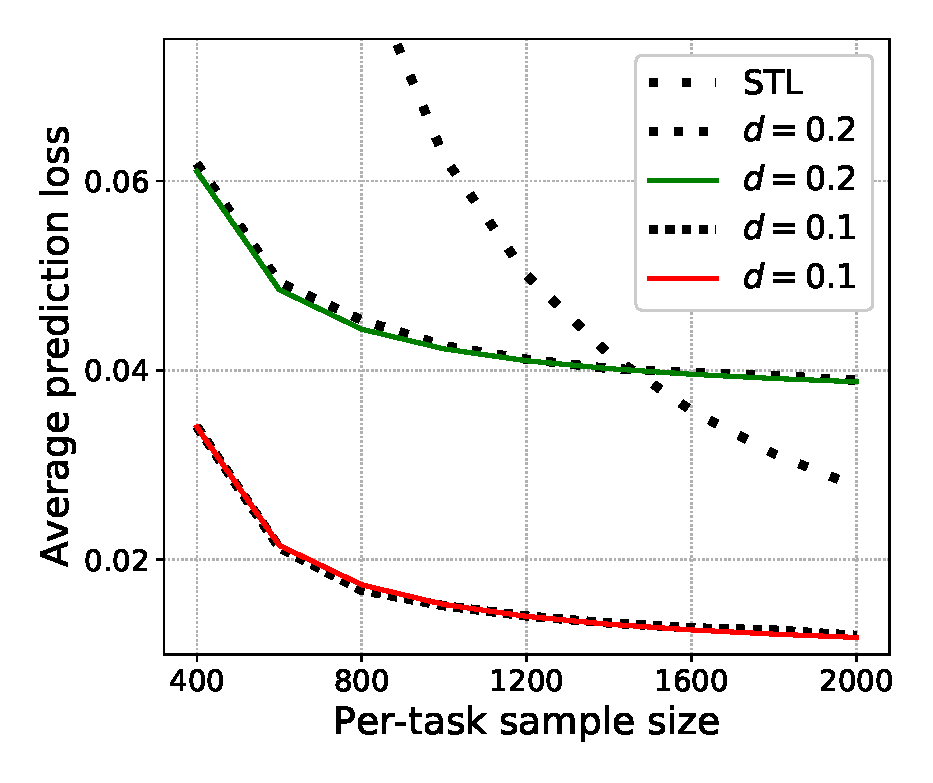
\includegraphics[width=0.9\textwidth]{figures/same_covariates.eps}
		\caption{Example \ref{ex_same_cov}}
		\label{fig_same_cov}
	\end{subfigure}\hfill
	\begin{subfigure}[b]{0.5\textwidth}
		\centering
		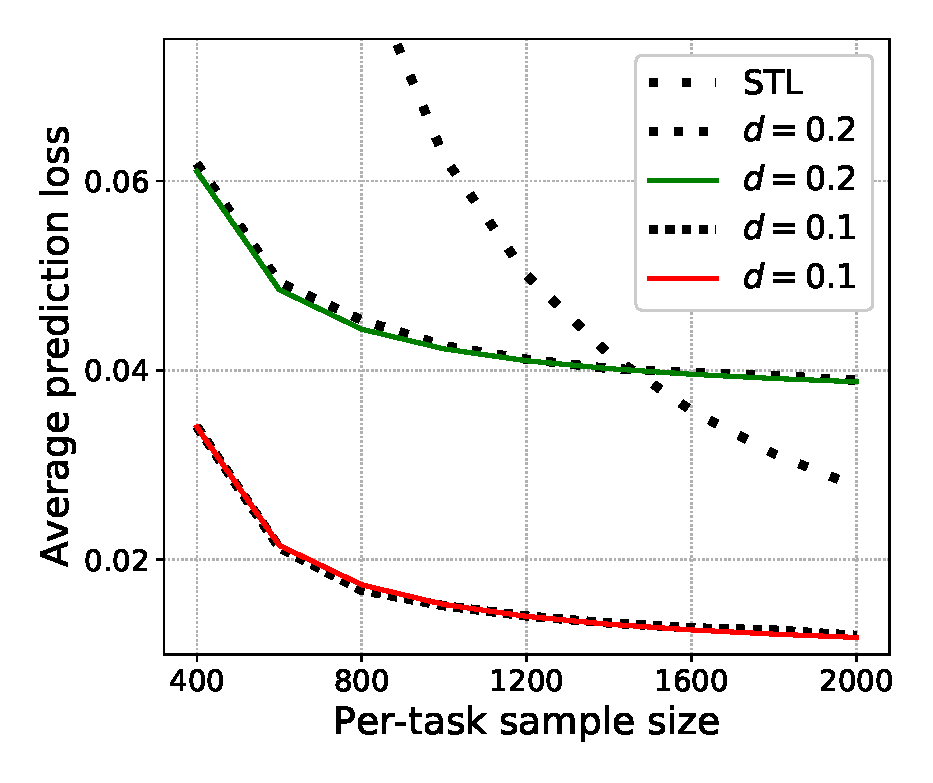
\includegraphics[width=0.9\textwidth]{figures/same_covariates.eps}
		\caption{Example \ref{ex_sample_ratio}}
		\label{fig_width}
	\end{subfigure}
%	\caption{%Three takeaways of our theory in Section \ref{sec_insight}.
%	Our estimated losses (solid line) match the empirical losses (dotted line) accurately under various settings in dimension $p = 200$.
%	\textbf{Left.} Validating Example \ref{ex_same_cov} for ten tasks: the noise variance $\sigma^2$ is $1/4$.
%	\textbf{Middle.} Validating Example \ref{ex_sample_ratio} for two tasks: we discover an interesting phenomena by fixing task two's sample size and increasing task one's sample size.
%	Moreover, our result accurately predicts the critical point (marked in circle) of the loss curve.
%	Depending on how large the distance $d^2$ is, task two's prediction loss decreases initially before increasing again, or decreases monotonically.
%	\textbf{Right.} We show how different levels of covariate shift affect hard parameter sharing when there is no bias.
%	Having covariate shift increases task two's prediction loss when task two's sample size is smaller than task one. Otherwise, having covariate shift (surprisingly) decreases task two's prediction loss.}
%	\label{fig_model_shift_phasetrans}
\end{figure*}

%Moreover, by setting $t=2$ in Theorem \ref{thm_many_tasks}, we can obtain the prediction loss for the HPS estimator for the transfer learning setting where the two tasks have the same covariates  $X^{(1)}=X^{(2)}$. For the reader's convenience, we give the precise statement in Corollary \ref{thm_two_tasks}.
%Theorem \ref{thm_many_tasks} implies Theorem \ref{thm_two_tasks} as a special case with $t=2$ and $r=1$.
%In this section, we consider the setting where the two tasks have the same covariates  $X^{(1)}=X^{(2)}$.
%We define $A^\star \in \R^{2}$ as the normalized eigenvector corresponding to the larger eigenvalue of the $2\times 2$ matrix
%$ {B^\star}^\top \Sigma  B^\star,$ where recall that $B^\star \define [{\beta}^{(1)},{\beta}^{(2)}] \in \real^{p\times 2}$ by definition.
% is the matrix formed by the linear model parameters of the two tasks.
%Without loss of generality, we assume that the two eigenvalues of ${B^\star}^\top \Sigma B^\star$ are not degenerate, so that $A^\star$ is uniquely defined. %Otherwise, Theorem \ref{thm_two_tasks} will give a null result.
%In the following corollary, the estimate \eqref{minimizer_beta1} shows that the minimizer $\hat a$ is approximately equal to $A^\star(1)/A^\star(2)$, while \eqref{Li_multi0} gives the exact asymptotic limit of $L_2(\hat{\beta}_2^{\MTL}(\hat a)) $, together with an explicit convergence rate that we believe to be sharp.

%\begin{corollary}\label{thm_two_tasks}
%Under Assumption \ref{assm_big1}, suppose that $X^{(1)}=X^{(2)}$ and $n_1=n_2\equiv n$. Let $c>0$ be an arbitrary (small) constant. Then we have that with high probability,
%\be\label{minimizer_beta1}
%\left\| u_{\hat a}u_{\hat a}^\top - A^\star {A^\star}^\top\right\|_F  \le  \left[\frac{ n^{-1/2+2/\varphi+c}  \|{B^{\star}}^{\top}\Sigma B^{\star}\|  + n^{-1/2+c} \sigma^2 }{\lambda_1 - \lambda_{2} } \right]^{1/2},
%\ee
%where $u_{\hat a}$ is the unit vector defined as
%$ u_{\hat a}:= \frac1{\hat a^2 +1} \begin{pmatrix} {\hat a}\\ %1\end{pmatrix},$ and $\lambda_1 $ and $\lambda_{2}$ are respectively the larger and smaller eigenvalues of ${B^\star}^\top\Sigma B^\star$.
%for task 2,  % over the randomness of the input,
%Moreover, the prediction loss of the HPS estimator satisfies that with high probability,
%	\begin{align}
%		& \bigabs{L_2(\hat{\beta}_2^{\MTL}(\hat a)) - \left\|(\Sigma^{(2)})^{1/2} \left(A^\star(2) \cdot B^{\star}A^{\star}  - \beta^{(2)}\right)\right\|^2  - |A^\star(2)|^2  \frac{p\sigma^2}{n-p} } \nonumber\\
%		& \le  \left[  \frac{  n^{-1/2+2/\varphi+c} \|{B^{\star}}^{\top}\Sigma B^{\star}\|+n^{-1/2+c} \sigma^2} {\lambda_1  - \lambda_2 }\right]^{1/2}   \left(\norm{\Sigma^{1/2} B^{\star}}^2+  \sigma^2\right), \label{Li_multi0}
		%\le n^{-\frac{c_{\varphi}}2} \cdot \frac{\bigbrace{ \norm{\Sigma^{1/2} B^{\star}}^2+  \sigma^2} \cdot (\bignormFro{\Sigma^{1/2} B^{\star}}^2 + \sigma^2 t)} {\lambda_r ({B^\star}^\top \Sigma B^\star)- \lambda_{r+1}({B^\star}^\top \Sigma B^\star)},
%	\end{align}
%	 where $A^\star(2)$ denotes the second entry of $A^\star$.
%	 \end{corollary}

\begin{example}%[Random-effect model]
\label{ex_same_cov}
%Suppose every $\beta^{(i)}$ consists of two random components, one that is shared among all tasks and one that is task-specific.
%Thus, each task contributes a certain amount to the shared component and injects a task-specific bias.
%More precisely, %we have
Suppose that {$\beta^{(i)}=\beta_0 +\wt \beta^{(i)}$} for $ i=1,2,\cdots, t,$
where $\beta_0$ denotes the shared component, %whose entries are i.i.d. Gaussian random variables of mean zero and variance $p^{-1}\kappa^2$,
and $\wt \beta^{(i)}$ denotes the $i$-th
%Let $\beta^{(i)}$ be equal to $\beta_0$ plus a
task-specific component whose entries are i.i.d. Gaussian random variables of mean zero and variance $p^{-1} d^2$.
%Thus, for any two different $\beta^{(i)}$ and $\beta^{(j)}$, their distance is roughly $2d^2$.
%The labels are $Y_i = X_i\beta_i + \varepsilon_i$, where $\e_i$ consists of i.i.d. entries with mean zero and variance $\sigma^2$.
%For our discussion below, we assume that $\kappa^2 \sim d^2 \sim \sigma^2$ and $n\sim p$. %and $d^2=\OO(\kappa^2)$.
%The more precise conditions on the relations between $d^2$, $\sigma^2$ and $\kappa^2$ are given in  \eqref{choiceofpara}.
%We assume that all the random variables have finite moments up to any order as in equation \eqref{assmAhigh2}.
In this random-effect model, using the concentration of Gaussian random vectors (e.g. Lemma \ref{largedeviation} in the supplement  \cite{MTL_suppl}),
%Based on the definition of the random-effect model,
the $(i, j)$-th entry of ${B^{\star}}^{\top} \Sigma B^{\star}$ is equal to %(ignoring lower order terms)
%\begin{align*}
%	\beta_i^{\top} \beta_j \approx \norm{\beta_0}^2 + \frac{d^2}{2}\delta_{ij},\quad 1\le i,j \le t,
%\end{align*}
\begin{align}\label{betaSbeta}
	\beta_i^{\top}\Sigma  \beta_j =\beta_0^\top \Sigma \beta_0 + \delta_{ij} \frac{d^2 }{p}\tr \Sigma + \OO\left(p^{-1/2+c}\|\beta_0\|^2+ p^{-1/2+c} d^2\right),
\end{align}
 with high probability for any constant $c>0$. We omit the details to show the error bound using Lemma \ref{largedeviation}.
%Note that $\norm{\beta_0}^2$ is approximately $\kappa^2$.
With \eqref{betaSbeta}, it is easy to calculate that with high probability, the eigenvalues of ${B^{\star}}^{\top} \Sigma B^{\star}$ are given by
$$\lambda_1=\left[1+\OO(p^{-1/2+c})\right]\cdot\left(t \beta_0^\top \Sigma \beta_0  + \frac{d^2}{ p}\tr \Sigma\right) ,$$
and
$$ \lambda_i=\left[1+\OO(p^{-1/2+c})\right]\cdot \frac{d^2}{ p}\tr \Sigma , \ \ i=2,\cdots, t.$$ %Therefore, by taking a rank-$1$ approximation of ${B^{\star}}^{\top} B^{\star}$, we get the average prediction loss of $B^{\star} a_i^{\star}$.
Thus for the best rank-$r$ approximation $A^\star {A^\star}^\top$  of ${B^{\star}}^{\top}\Sigma  B^{\star}$, we have
$$\bignorm{\Sigma^{1/2} B^{\star} (A^\star {A^\star}^{\top} - \id_{t\times t})}_F^2= [1+\OO(p^{-1/2+c})]\cdot(t-r)\frac{d^2}{ p}\tr \Sigma $$
with high probability.
%To see this, recall that $r$ is one and $A^{\star} {A^{\star}}^{\top}$ is the best rank-$1$ approximation of ${B^{\star}}^{\top}\Sigma B^{\star} = {B^{\star}}^{\top} B^{\star}$.
%Hence, the above expression is equal to the sum of ${B^{\star}}^{\top} {B^{\star}}$'s bottom $t-1$ singular values.
%In the random-effect model described above, we further assume that $\Sigma$ is isotropic as an example.
%We show that when the rank $r$ is one, the average prediction loss of hard parameter sharing is as follows
Then using \eqref{Li_multi2}, we obtain that
\[ \frac{1}{t}\sum_{i=1}^t L_i(\hat{\beta}_i^{\MTL}) = \bigbrace{1 - \frac{r}{t}} \frac{d^2}{p}\tr \Sigma + \frac{r}{t} \cdot \frac{p\sigma^2 }{n - p} +\oo(\|\beta_0\|^2+d^2 + \sigma^2) ,\quad \text{w.h.p. }\]
%We describe a proof sketch.
%First, we show that the bias equation $L(B^{\star} a_i^{\star})$ simplifies to the following
%\[ \frac{1}{t} \sum_{i=1}^t L(B^{\star} a_i^{\star}) = \frac{1}{t}\normFro{B^{\star} A^{\star} {A^{\star}}^{\top} - B^{\star}}^2 \approx \left(1 - \frac{1}{t}\right) {d^2}{}  . \]
%Second, using Fact \ref{fact_tr}, one can see that the average variance is
%\begin{align*}
%	\frac{1}{t} \sum_{i=1}^t \sigma^2\norm{a_i^{\star}}^2 \bigtr{\Sigma (X^{\top} X)^{-1}} = \frac{\sigma^2}{t} \sum_{i=1}^t \norm{a_i^{\star}}^2 \frac{p}{n - p}
%	= \frac{1}{t}\frac{\sigma^2 p}{n - p},
%\end{align*}
%because $A^{\star}$ has rank-$1$ and $\sum_{i=1}^t \norm{a_i^{\star}}^2 = 1$.
%Combined together, we have derived the average prediction loss in the random-effect model.
%If the error is sufficiently small, then
Comparing the above equation with \eqref{L_STL_simple01} (and ignoring the small error), we have the following observations.
%Recall that the average prediction loss of STL scales as $\sigma^2\cdot \bigtr{\Sigma (X^{\top} X)^{-1}} = \frac{\sigma^2 p}{n - p}$ by Fact \ref{fact_tr}.
%Comparing HPS to STL, we have the following qualitative properties.
%	Suppose $n$ is sufficiently large so that the error is negligible.
%\begin{enumerate}
\begin{enumerate}
	\item {\bf Positive vs. negative transfer.} The averaged HPS prediction loss is smaller than the single-task OLS prediction loss if and only if $\frac{d^2}{p}\tr \Sigma  < \frac{p\sigma^2 }{n - p}$, that is, the ``task-specific variance'' is smaller than the ``noise variance'' up to some constant factor.

	\item {\bf The optimal rank $r$.} If $\frac{d^2}{p}\tr \Sigma  < \frac{\sigma^2 p}{n - p}$, then the smallest averaged HPS  prediction loss is achieved when $r=1$. Hence increasing the width $r$ of the shared feature representation layer does not help.
	%To see this, one can verify what when $r$ increases by one, bias reduces by $\frac{d^2}{t}$, but variance increases by $\frac{\sigma^2 p}{t(n-p)} > \frac{d^2}{t}$ (details omitted).


%	\item {\bf Sample efficiency.} Suppose $\frac{d^2}{p}\tr \Sigma  < \frac{\sigma^2 p}{n - p}$ and we choose the optimal rank $r=1$. Following \FY{add citation}, we define the data efficiency ratio of HPS as the proportion of labelled data needed to achieve comparable performance to single-task linear regression. More precisely, for some $x\in (0,1)$, if we only use $xn$ many data, then the averaged HPS predication loss is
%	\[ \frac{1}{t} \sum_{i=1}^t L_i(\hat{\beta}_i^{\MTL},x) = \bigbrace{1 - \frac{1}{t}} \frac{d^2}{p}\tr \Sigma  + \frac{1}{t} \cdot \frac{p\sigma^2 }{xn - p}+\oo(d^2 + \sigma^2) ,\quad \text{with high probability. }\]
%	Comparing it to the single-task OLS predication loss $t^{-1} \sum_{i=1}^t L_i(\hat{\beta}_i^{\STL})$, we find that HPS requires at most (recall that $\rho=n/p$)
%	$$x= \frac{1}{\rho} + \frac{1 - \rho^{-1}}{t - (t - 1)(\rho-1)\frac{d^2 }{\sigma^2 } \cdot \frac1p\tr\Sigma}$$
%	proportion of the samples to achieve the same performance. This is the data efficiency ratio for the above random-effect model.
	%samples that is less than $n$ samples to get comparable loss to STL.
	%This follows by using this sample size in the average prediction loss equation in Example \ref{ex_same_cov}.
	\end{enumerate}
\end{example}



%We demonstrate the accuracy of our results in simulations.
%While our theory is asymptotic (with error terms that are negligible when $p$ is sufficiently large), we observe that they are incredibly accurate in a moderate dimension of $p = 200$.



First, we validate the result of Example \ref{ex_same_cov}.
Figure \ref{fig_same_cov} shows the average prediction loss over ten tasks as we increase the number of samples per-task from $400$ to $2000$.
In all the parameter settings, our results estimate the empirical losses accurately.
We also observe a trend that the average prediction loss increases as we increase distance $d$ from $0.1$ to $0.2$.
Our work explains the differences between these two settings since $d^2 = 0.1^2$ is always smaller than $\frac{\sigma^2 p}{n - p}$, but $d^2 = 0.2^2$ is not.
%Second, when $d = 0.1$, we have that $d^2 \le \frac{\sigma^2 p}{n - p}$ for all values of $n$, hence the average prediction loss of hard parameter sharing is always lower than STL.
Indeed, we observe a crossover point between hard parameter sharing and STL.
Finally, for $d = 0.2$, looking horizontally, we find that HPS requires fewer samples per-task than STL to achieve the same loss level. %\FY{I do not quite understand this sentence about "3x fewer", because how much data needed depends on $d$ and the prediction loss level we are looking at. For example, at the cross point, this ratio is 1. }


%Our result from Corollary \ref{cor_MTL_loss} explains this trend.


%Covariate shift: We set $\kappa = 1$ and $d = 0$.
%We set $\rho_2 = 4$ and vary $\rho_1$ from $5$ to $25$ for sample sizes.
%We use the scale parameter $\lambda = 1$ for the curve without covariate shift and $\lambda = 2$ for the curve with covariate shift (cf. Section \ref{sec_covshift}).


%Recall that Section \ref{sec_data_size} shows that increasing the data size of the source task does not always improve the performance of MTL for the target task.
%In Figure \ref{fig_ab_data}, we show that for source task MR and target task SST, there is a transition from positive to negative transfer as we increase the data size of the source task.
%Our result provides a fine-grained insight on the covariance alignment algorithm proposed in \cite{WZR20}.
%Recall that the covariance alignment procedure in \cite{WZR20} adds an additional module between the word embedding representation and the shared module.
%When the source task data size is particularly large compared to the target task, we show that applying the covariance alignment algorithm results in more significant gains.
%In Figure \ref{fig_ab_cov}, we observe that the benefit from aligning task covariances becomes more significant for LSTM and MLP as we increase the number of datapoints of the source task.

%\begin{table}
%	\begin{center}
%		\begin{tabular}{c c c c c}
%			\toprule
%			\multirow{2}{*}{{\bf Models}} & \multicolumn{2}{c}{\begin{minipage}{1.1in}\begin{center}
%				                                                                          MR, SST, SUBJ, CR, MPQA, TREC\end{center}\end{minipage}} & \multicolumn{2}{c}{\begin{minipage}{1.1in}\begin{center}MR, SST, SUBJ, CR, MPQA\end{center}\end{minipage}} \\
%			\cmidrule(lr){2-3} \cmidrule(lr){4-5}
%			& {\bf Stanford} & {\bf Alignment} & {\bf Stanford} & {\bf Alignment} \\
%			\midrule
%			{\bf MLP}  & > 100\% & 39\% & 25\% & 25\% \\
%			{\bf LSTM} & 36\% & 36\% & 28\% & 25\% \\
			% {\bf CNN}  & 76\% & - & 32\% & -\\
%			\bottomrule
%		\end{tabular}
%	\end{center}
%	\caption{Taskonomy experiment.}
%	\label{tab:taskonomy}
%\end{table}
%\begin{figure}[!t]
%	\centering
%	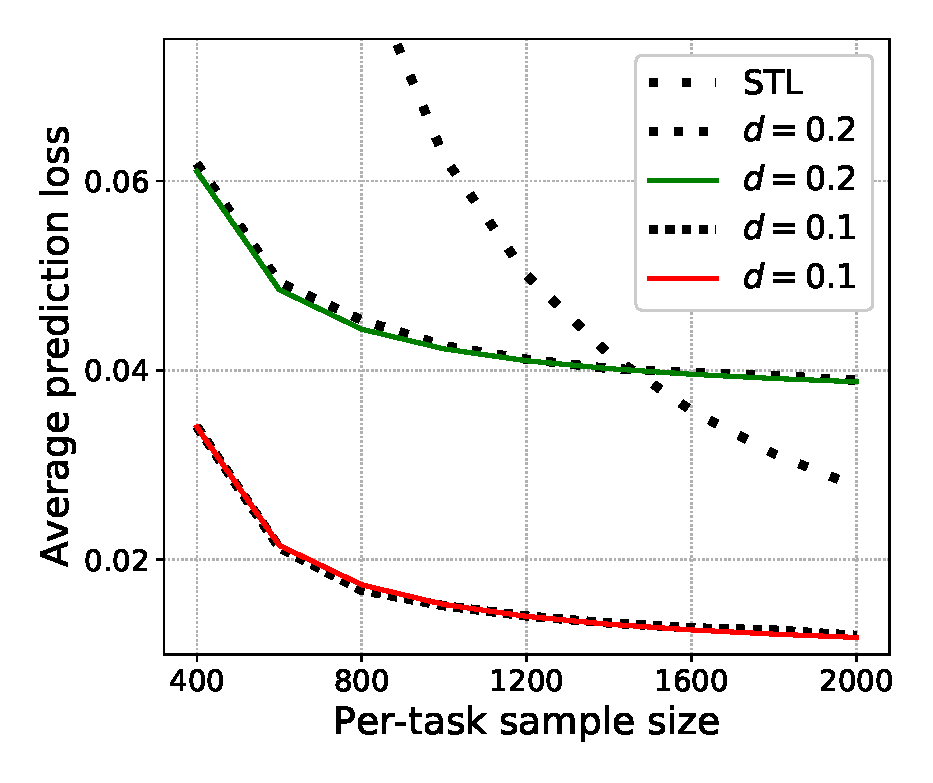
\includegraphics[width=0.35\textwidth]{figures/same_covariates.eps}
%	\caption{Validating Example \ref{ex_same_cov} in Section \ref{sec_same} for $10$ tasks: our estimated loss (solid line) matches the empirical loss (dotted line) accurately for various task-specific variance $d^2$ and sample size $n$ settings. The feature dimension $p$ is $200$, and noise variance $\sigma^2$ is $1/4$.}
%	\label{fig_same_cov}
%\end{figure}





%The estimate \eqref{minimizer_beta1} shows that the minimizer $\hat a$ is approximately equal to $A^\star(1)/A^\star(2)$, while \eqref{Li_multi0} gives the exact asymptotic limit of $L_2(\hat{\beta}_2^{\MTL}(\hat a)) $, together with an explicit convergence rate that we believe to be sharp.


%It is not hard to extend the above result to the cases with more than two tasks. We make this extension for the following reasons. First, it provides a clearer geometric intuition than the two-task setting as we will discuss below. Second, the corresponding multi-task setting is prevalent in applications of multi-task learning to image classification, where there are multiple prediction labels/tasks for every image \cite{chexnet17,EA20}. Finally, it provides useful insights into a more general theory of multi-task learning, which we will explore in greater details in future works.

%We consider an arbitrary local minimum $B, W_1, \dots, W_2$ of the optimization objective.
%We extend the bias-variance decomposition from the two-task case to the multiple-task case.
%We observe that the expected prediction loss of $\hat{\beta}_t^{\MTL}$ conditional on $X$ consists of a bias and a variance equation as follows
%\begin{align}
%	\exarg{\varepsilon_1, \dots, \varepsilon_t}{L(\hat{\beta}_t^{\MTL}) \mid X}
%	=& \bignorm{\Sigma^{1/2} \bigbrace{B^{\star} \cW^{\top} (\cW \cW^{\top})^{-1} W_t - \beta_t}}^2 \label{eq_bias_multiple} \\
%	&+ \sigma^2 \cdot (W_t^{\top} (\cW \cW^{\top})^{-1} W_t) \cdot \bigtr{\Sigma (X^{\top} X)^{-1}} \label{eq_var_multiple}
%\end{align}
%One can see that equation \eqref{eq_bias_multiple} is the bias of the multi-task learning estimator and equation \eqref{eq_var_multiple} is its variance.
%Compared to the prediction loss of single-task learning (cf. equation \eqref{eq_var_stl}), we observe that the variance equation \eqref{eq_var_multiple} is always smaller because $W_t^{\top} (\cW \cW^{\top})^{-1} W_t \le 1$.
%On the other hand, the bias equation \eqref{eq_bias_multiple} is always larger because of the difference between the task models.
%We show the generalization error of hard parameter sharing estimators.
%Before stating the result, we define the following notations.




%The key step for proving Theorem \ref{thm_many_tasks} is a characterization of $f(A, B)$'s global minimizer.
%\medskip
%
%\noindent\textbf{Comparison to single-task learning (STL).}
%Theorem \ref{thm_many_tasks} provides a sharp generalization error bound that is asymptotically tight when $n$ goes to infinity.
%%The limiting loss of hard parameter sharing consists of two parts, a bias term $L(B^{\star} a_i^{\star})$ that measures the error of $B^{\star} a_i^{\star}$, and a variance term that scales with noise variance $\sigma^2$.
%%	Our result implies that the variance of hard parameter sharing is always smaller than single-task learning.
%%	This is because	STL's variance is equal to $\frac{\sigma^2 \cdot p} {n - p}$ by Fact \ref{lem_minv}, and $\norm{a_i^{\star}}^2 \le 1$ since the spectral norm of $U_r$, which is a projection matrix, is at most one.
%One direct implication of our result is that compared to STL, the variance always decreases, since STL's variance is equal to $\sigma^2 \tr[\Sigma (X^{\top} X)^{-1}]$.
%On the other hand, the bias always increases.


%\FY{add simulations to check our results; discuss motivations and possible applications}
\iffalse
In this paper, we consider a natural extension of the estimator $\hat \beta^{\rm{TL}} $, that is, the \emph{hard parameter sharing} (HPS) estimator, which has been a standard type of estimator in multi-task learning \FY{citations}. More precisely, we study the following HPS architecture: a shared feature representation layer $B\in\real^{p}$ for all datasets and a separate output layer $A_i \in \real$ for every dataset $i$. Then we study the following minimization problem:
\begin{align}\label{eq_tsl}
			f(A, B) = \norm{X^{(1)} B A_1 - Y^{(1)}}^2 + \norm{X^{(2)} B A_2 - Y^{(2)}}^2,
\end{align}
where we abbreviate $A = [A_1, A_2]$. Let $(\hat{A}, \hat{B})$ be the minimizer of $f(A, B)$. We define the hard parameter sharing (HPS) estimator for task $i$ as
\be\label{def_HPS}\hat{\beta}_i^{\MTL} = \hat{B} \hat{A}_i,\quad i=1,2.\ee
Note that $\hat \beta^{\rm{TL}}$ is a special case of $\hat{\beta}_i^{\MTL}$ by setting $A_1=A_2=1$.

For the optimization objective $f(A, B)$ in \eqref{eq_tsl}, using the local optimality condition $\frac{\partial f}{\partial B} = 0$, we can solve that
	\begin{align}
		\hat{B} = A_2^{-1} \hat \Sigma(a)^{-1} \left[a (X^{(1))})^{\top}Y^{(1)} +  (X^{(2)})^{\top}Y^{(2)}\right], \label{eq_Bhat_2task} %\\
		%&= (B^\star A ^{\top}) (A A^{\top})^{-1} + (X^{\top}X)^{-1}X^{\top}   \bigbrace{\sum_{j=1}^t \varepsilon_i A_i^{\top}} (A  A^{\top})^{-1}.
	\end{align}
where we denote $a:=A_1/A_2$ and $\hat \Sigma(a):= a^2 (X^{(1)})^\top X^{(1)}  + (X^{(2)})^\top X^{(2)}$.
Applying $\hat B$ to equation \eqref{eq_tsl}, we obtain an objective that only depends on $a $ as follows %\HZ{$A$ has been used to denote the output layers. Could you replace $A$ with another symbol (say $x$)?}
 \begin{align}
		 g(a) \define & \left\| X^{(1)} \hat\Sigma(a)^{-1} (X^{(2)})^\top X^{(2)} (a\beta^{(2)}-\beta^{(1)}) \right. \nonumber\\
			& \left. + \left(a^2 X^{(1)}\hat \Sigma(a)^{-1} (X^{(1)})^\top-\id_{n_1\times n_1}\right)\epsilon^{(1)}+ a X^{(1)}\hat \Sigma(a)^{-1} (X^{(2)})^\top \epsilon^{(2)} \right\|^2 \nonumber\\
		   +& \left\| X^{(2)} \hat \Sigma(a)^{-1} (X^{(1)})^\top X^{(1)} (a\beta^{(1)}-a^2\beta^{(2)}) \right. \nonumber\\
		  &\left.+ \left(X^{(2)}\hat\Sigma(a)^{-1} (X^{(2)})^\top-\id_{n_2\times n_2}\right)\epsilon^{(2)} + a X^{(2)}\hat \Sigma(a)^{-1} (X^{(1)})^\top \epsilon^{(1)} \right\|^2. \label{eq_mtl_A12}
	\end{align}
Let $\hat a$ be the minimizer of $g(a)$. Throughout this paper, we regard $Y^{(1)}$ as the source data, and $Y^{(2)}$ as the target data.  Then the HPS estimator \eqref{def_HPS} for the target task 2 is
\be\label{HPS_est}
\hat{\beta}_2^{\MTL} (\hat a) = \hat \Sigma(\hat a)^{-1}  \left[\hat a (X^{(1))})^{\top}Y^{(1)} +  (X^{(2)})^{\top}Y^{(2)}\right].
\ee
\fi
